% The Clever Algorithms Project: http://www.CleverAlgorithms.com
% (c) Copyright 2013 Jason Brownlee. Some Rights Reserved. 
% This work is licensed under a Creative Commons Attribution-Noncommercial-Share Alike 2.5 Australia License.


% Name
% The algorithm name defines the canonical name used to refer to the technique, in addition to common aliases, abbreviations, and acronyms. The name is used in terms of the heading and sub-headings of an algorithm description.
\section{Locally Estimated Scatterplot Smoothing} 
\label{sec:loess}
\index{Locally Weighted Regression}
\index{Locally Weighted Polynomial Regression}
\index{LOESS}
\index{LOWESS}
\index{Locally Estimated Scatterplot Smoothing}
\index{Locally Weighted Scatterplot Smoothing}

% other names
% What is the canonical name and common aliases for a technique?
% What are the common abbreviations and acronyms for a technique?
\emph{Locally Estimated Scatterplot Smoothing, LOESS, Locally Weighted Regression, LWR, Locally Weighted Polynomial Regression.}

% Taxonomy: Lineage and locality
% The algorithm taxonomy defines where a techniques fits into the field, both the specific subfields of Computational Intelligence and Biologically Inspired Computation as well as the broader field of Artificial Intelligence. The taxonomy also provides a context for determining the relation- ships between algorithms. The taxonomy may be described in terms of a series of relationship statements or pictorially as a venn diagram or a graph with hierarchical structure.
\subsection{Taxonomy}
% To what fields of study does a technique belong?
Locally Estimated Scatterplot Smoothing (LOESS) is a type of Local Regression and belongs to the general class of Non-Parametric Regression methods. It also belongs to the framework of Generalized Additive Models (GAMs).
% What are the closely related approaches to a technique?
LOESS is an extension to its precursor method Locally Weighted Scatterplot Smoothing (LOWESS).
It is related to other Non-Parametric Regression methods such as Multivariate Adaptive Regression Splines (MARS), Non-Parametric Multiplicative Regression, Additive Regression Model and Regression Trees. 

% Strategy: Problem solving plan
% The strategy is an abstract description of the computational model. The strategy describes the information processing actions a technique shall take in order to achieve an objective. The strategy provides a logical separation between a computational realization (procedure) and a analogous system (metaphor). A given problem solving strategy may be realized as one of a number specific algorithms or problem solving systems. The strategy description is textual using information processing and algorithmic terminology.
\subsection{Strategy}
% What is the information processing objective of a technique?
The information processing objective of the technique is to find an equation that best describes the relationships between independent and a dependent variable.
% What is a techniques plan of action?
This is achieved by fitting a local low-order polynomial model to nearby points, where `nearby' is defined by a distance kernel function (such as a nearest neighbor Euclidean distance kernel for continuous variables) between observations. A given polynomial model is fit using weighted least squares as needed,  where the response point is used as the centroid for the distance kernel function. The amount of data used to fit each local model is called the bandwidth or smoothing parameter. Regression models are created just-in-time for each response that is required.

% Heuristics: Usage guidelines
% The heuristics element describe the commonsense, best practice, and demonstrated rules for applying and configuring a parameterized algorithm. The heuristics relate to the technical details of the techniques procedure and data structures for general classes of application (neither specific implementations not specific problem instances). The heuristics are described textually, such as a series of guidelines in a bullet-point structure.
\subsection{Heuristics}
% What are the suggested configurations for a technique?
% What are the guidelines for the application of a technique to a problem instance?

\begin{itemize}
	\item LOESS is very simple, requiring only a sample of data to compute a local model for a given observation.
	\item The method delays computation until the time a response is needed, although computation at this time can be relatively demanding.
	\item The method is well suited to problems of time series prediction and two-dimensional data exploration (by projecting the line on a scatter plot of the data).
	\item It is common set the bandwidth parameter used to fit a local model using 25\% to 50\% of the given training dataset.
	\item It is common to use low order polynomials as local models, typically first (linear) or second (quadratic) degree. Higher order polynomials are expected to over-fit the data.
	\item It performs is as good as the training data, requiring relatively large non-sparse datasets (good local structure) to produce good predictions.
	\item It does not produce a single equation model like OLS that can be analyzed and understood.
\end{itemize}

% sample script in R
\subsection{Code Listing}
% listing
Listing~\ref{stats_locally_estimated_scatterplot_smoothing} provides a code listing of the Locally Estimated Scatterplot Smoothing method in R.
Figure~\ref{plot:locally_estimated_scatterplot_smoothing_result} provides a plot of the training dataset with the line of best fit highlighted.

% algorithm and package
The example uses the \texttt{loess()} function in the \texttt{stats} core package that provides Local Polynomial Regression Fitting using the LOESS method \cite{RDCT2011a}. For more information on this library type: \texttt{library(help="stats")}, and for more information on the function type: \texttt{?loess}.

% problem
The test problem is a two-dimensional dataset of 50 samples, where the \texttt{x}-values are drawn from a uniformly random distribution $x \in [0,10]$ and \texttt{y} values are the \texttt{x} value plus a value drawn from a normally random distribution with a mean of $0$ and a standard deviation of $1$.

% code listing
\lstinputlisting[firstline=7,language=r,caption={Example of Locally Estimated Scatterplot Smoothing in R using the \texttt{loess} function of the \texttt{stats} core package.}, label=stats_locally_estimated_scatterplot_smoothing]{../src/algorithms/regression/stats_locally_estimated_scatterplot_smoothing.R}

\begin{figure}[htp]
\centering
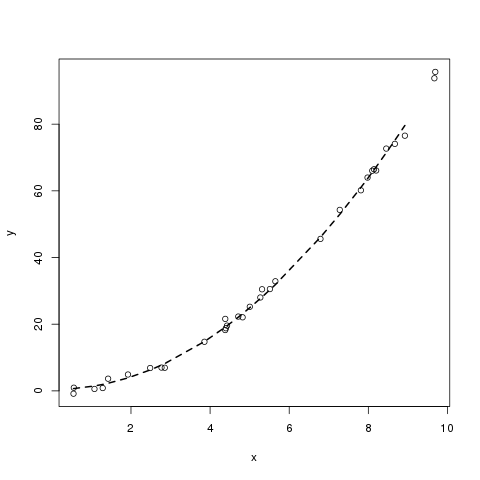
\includegraphics[scale=0.45]{a_regression/locally_estimated_scatterplot_smoothing_result.png}
\caption{Plot 2D showing the predicted line of best fit for the test dataset.}
\label{plot:locally_estimated_scatterplot_smoothing_result}
\end{figure}

% other packages
The \texttt{stats} package also provides an implementation of LOWESS in the \texttt{lowess()} function.

% References: Deeper understanding
% The references element description includes a listing of both primary sources of information about the technique as well as useful introductory sources for novices to gain a deeper understanding of the theory and application of the technique. The description consists of hand-selected reference material including books, peer reviewed conference papers, journal articles, and potentially websites. A bullet-pointed structure is suggested.
\subsection{References}
% What are the primary sources for a technique?
% What are the suggested reference sources for learning more about a technique?

% primary sources
\subsubsection{Primary Sources}
% precursor
Cleveland described a form of univariate local regression called Locally Weighted Scatterplot Smoothing (LOWESS) which also included a robust version of the method \cite{Cleveland1978, Cleveland1979}. 
This method was extended to the multivariate case by Devlin in an unpublished technical report \cite{Devlin1986}.
% seminal
Locally Estimated Scatterplot Smoothing (LOESS) or Multivariate Locally Weighted Regression is credited to Cleveland and Devlin \cite{Cleveland1988}.

% more info
\subsubsection{More Information}
% precursor
Cleveland presented a FORTRAN routine for LOWESS for data exploration \cite{Cleveland1981}.
% follow-ups
LOESS was further described by Cleveland et~al.\ \cite{Cleveland1988a}.
% implementation
LOESS was further developed by Cleveland and Grosse \cite{Cleveland1991} and later well described in terms of an implementation in S (Rs pre-cursor) \cite{Cleveland1992}.
% modern
Cleveland and Loader provide a more recent salient description of local regression including the history of the general method and examples \cite{Cleveland1996}.
Atkeson et~al.\ provide a broader survey of the field of locally weighted learning methods (lazy or memory-based learning), focusing on locally weighted linear regression \cite{Atkeson1997}.

% END
